%% ==============================
\chapter{\iflanguage{ngerman}{Methoden}{Methods}}
\label{sec:methods}
%% ==============================



Im Paper von Hong \cite{hong2003method} wird ein Approximationsbasiertes Verfahren zur Berechnung von Gradienten eines Volumens vorgestellt. 
\newline
Hierbei ist zu beachten, dass der Gradient nicht für einen Voxel direkt berechnet werden kann. Der Gradient liegt im Falle eines dreidimensionalen Volumens im Zentrum eins Würfels, der von 4 benachbarten Voxeln aufgepsannt wird. In Hongs Verfahren wird zur Berechnung die lokale 4x4x4 Nachbarschaft hinzugezogen.
\newline
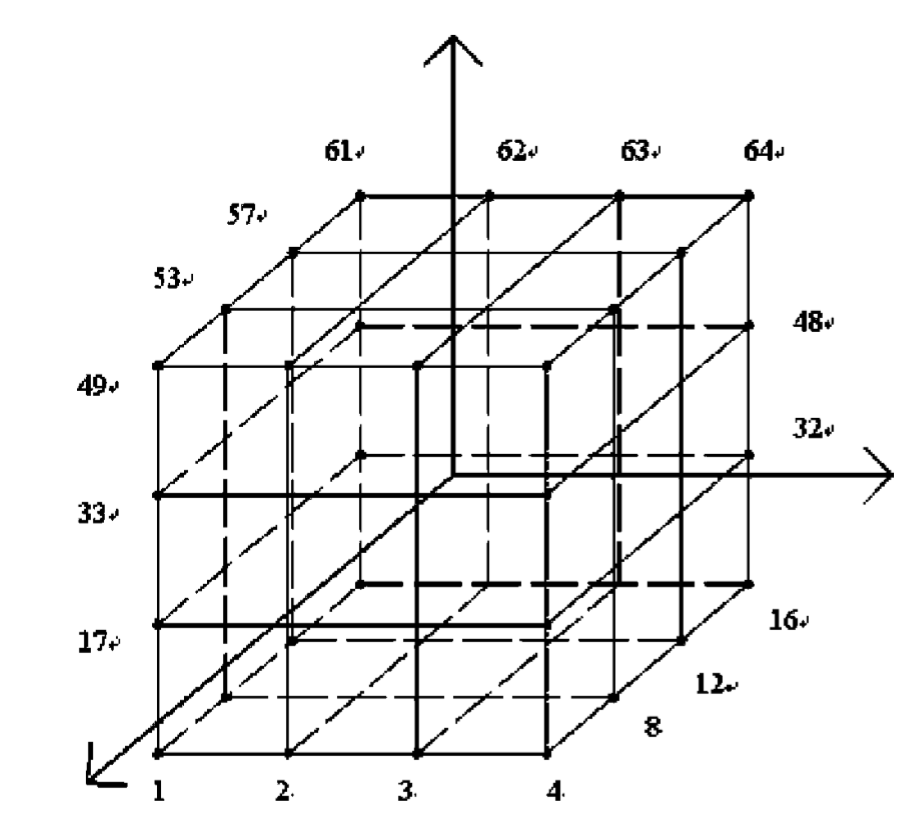
\includegraphics[width=\textwidth]{Logos/VoxelEdges.PNG}
\todo{richtig bild zitieren u. evtl kleiner}

Die Funktionen für die Intensitätswerte wird im Paper mit:  $f(x,y,z) = Ax^{2}+By^{2}+Cz^{2}+2Fyz+2Gzx+2Hxy+2Ix+2Jy+2Kz+D$  approximiert. Den dreidimensionalen Gradientenvektor n erhält man, indem man die Funktion ableitet: $n = (Ax+Gz+Hy+I, By+Fz+Hx+J, Cz + Fy + Gx + K)$ .
\newline
Um den Gradienten zu Berechnen müssen die Parameter A,B,C,E,F,G,H,I,J,K  berechnet werden. Dies geschieht mithilfe der Methode der kleinsten Quadrate.